By Section \ref{Numerical methods for computing the Casimir energy}, to compute the Casimir energy, it is necessary to evaluate the term
$\log\frac{\det\mathsf{V}_{\mathrm{i}k}}{\det\tilde{\mathsf{V}}_{\mathrm{i}k}} = \log\det(\mathsf{V}_{\mathrm{i}k}\tilde{\mathsf{V}}_{\mathrm{i}k}^{-1})$ 
with different values of $k$. In this section, several efficient methods will be introduced to compute this log determinant.

The log determinant of the matrix $\mathsf{V}_{\mathrm{i}k}\tilde{\mathsf{V}}_{\mathrm{i}k}^{-1}$ is equal to the sum of the logarithm of the eigenvalues of 
$\mathsf{V}_{\mathrm{i}k}\tilde{\mathsf{V}}_{\mathrm{i}k}^{-1}$. Since $\tilde{\mathsf{V}}_{\mathrm{i}k}$ is a compact perturbation of $\mathsf{V}_{\mathrm{i}k}$,
most of the eigenvalues of the matrix $\mathsf{V}_{\mathrm{i}k}\tilde{\mathsf{V}}_{\mathrm{i}k}^{-1}$ are close to 1 
(shown in the Figure \ref{eigenvalues of VVtilde}) and contribute little on the value of Casimir energy.
Therefore, the computation process for the large-scale problem can become efficient if only multiple extreme eigenvalues 
that mainly contribute to the log determinant are computed. In addition, we should also avoid directly computing the inverse of the matrix $\tilde{\mathsf{V}}_{\mathrm{i}k}$
since the computational complexity is cubic with respect to the matrix dimension.

In what follows, one method called inverse-free Krylov subspace method will be introduced to computed multiple extreme eigenvalues. For each quadrature point
$k_{j}$, $j = 1, \dots, N$, one can directly apply this method to find the log determinant of 
$\mathsf{V}_{\mathrm{i}k_{j}}\tilde{\mathsf{V}}_{\mathrm{i}k_{j}}^{-1}$. However, by recalling Figure 
\ref{The integrand decays exponentially}, most of the quadrature points are closed to each other, which inspires us to recycle the subspace obtained from 
$\mathsf{V}_{\mathrm{i}k_{j}}\tilde{\mathsf{V}}_{\mathrm{i}k_{j}}^{-1}$ and use it for $\mathsf{V}_{\mathrm{i}k_{j+1}}\tilde{\mathsf{V}}_{\mathrm{i}k_{j+1}}^{-1}$'s case.
Afterwards, another efficient method based on the standard Arnoldi iterations will be demonstrated and its corresponding recycling-subspace-based method will be discussed as well.
Finally, the comparison of among these methods on their performance for approximating the log determinant and the number of matrix-vector multiplications 
will be shown.
\begin{figure}[H]
    \centering
    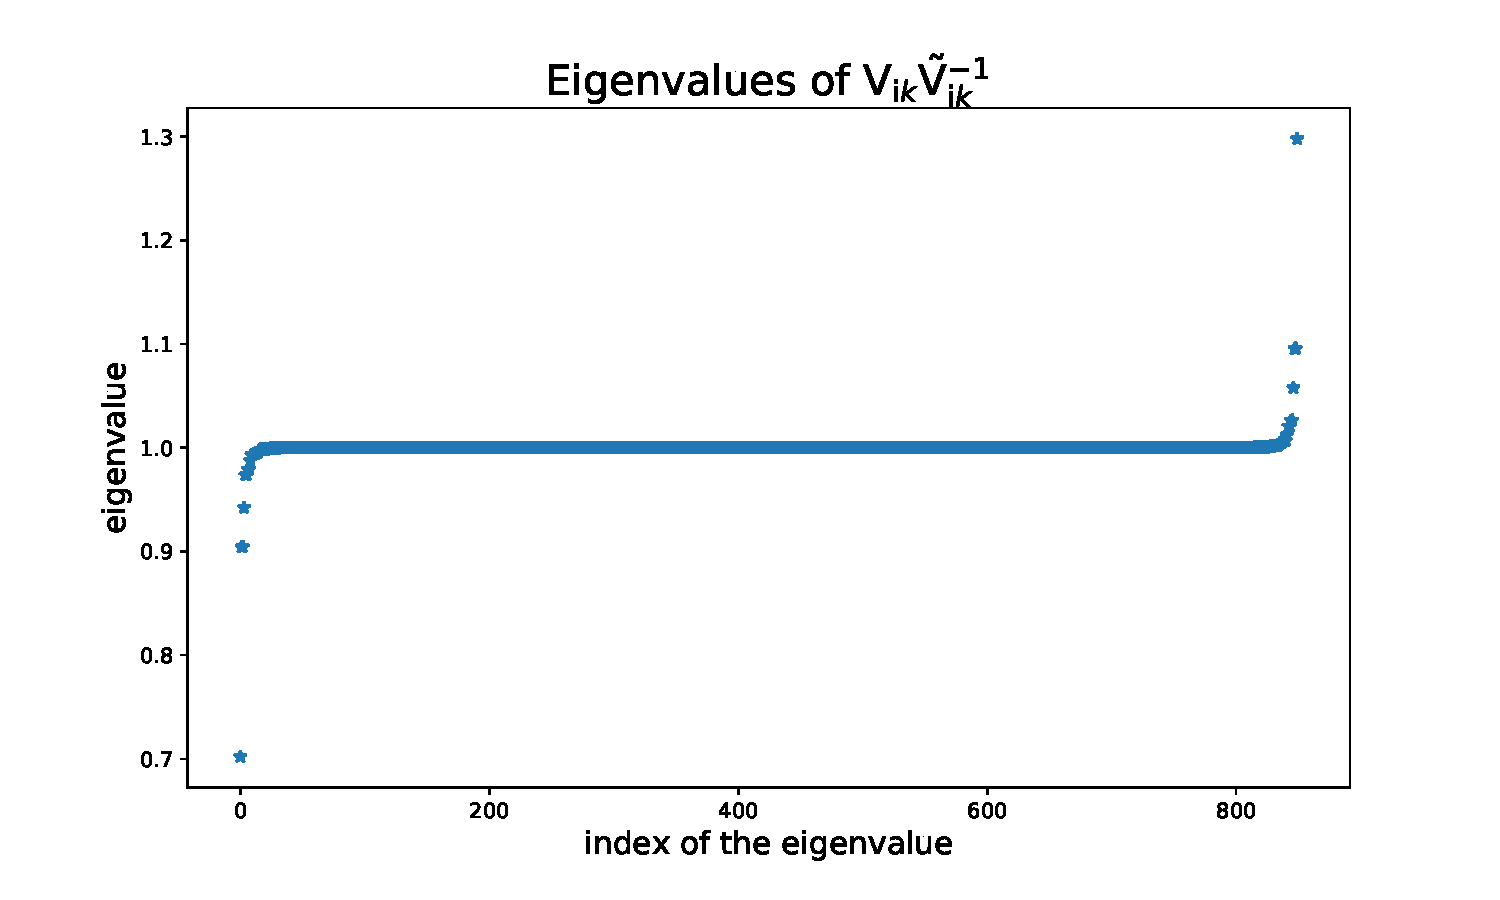
\includegraphics[scale = 0.5]{figures/eigenvalue_of_VVtilde.pdf}
    \caption{The eigenvalues of the matrix $\mathsf{V}_{\mathrm{i}k}\tilde{\mathsf{V}}_{\mathrm{i}k}^{-1}$ when $\mathrm{i}k = 0.8\mathrm{i}$.
    The scatterers are two spheres with equal radii $r_{1} = r_{2} = 1$ and the minimal distance between them is $Z = 0.5$. The grid size of the mesh is $h = 0.1$.}
    \label{eigenvalues of VVtilde}
\end{figure}
\subsection{Method I: Inverse-free Krylov subspace method}
Consider the eigenvalue problem: 
\begin{align} \label{EP}
    \mathsf{V}_{\mathrm{i}k}\tilde{\mathsf{V}}_{\mathrm{i}k}^{-1}\boldsymbol{x} = \lambda\boldsymbol{x},
\end{align}
where $\lambda$ is the eigenvalue and $\boldsymbol{x}$ is the corresponding eigenvalue. This eigenvalue problem is equivalent to the following generalized eigenvalue problem:
\begin{align}\label{GEP}
    \mathsf{V}_{\mathrm{i}k}\tilde{\boldsymbol{x}} = \lambda \tilde{\mathsf{V}}_{\mathrm{i}k}\tilde{\boldsymbol{x}}.
\end{align}
Thus, we can focus on solving the problem \eqref{GEP} instead of \eqref{EP} to avoid computing the matrix inversion. By \cite{golub2002inverse}\cite{money2005algorithm},
the authors proposed an inverse-free Krylov subspace method for computing a few extreme eigenvalues of the symmetric definite generalized eigenvalue problem 
and the following algorithm summarizes this method.

\begin{algorithm}[H]
    \SetAlgoLined
    Input: Symmetric matrix $A\in\mathbb{R}^{n\times n}$, s.p.d matrix $B\in\mathbb{R}^{n\times n}$, an initial approximation $\boldsymbol{x}$ with $||\boldsymbol{x}|| = 1$,
    the shift $\rho = 1$ and the dimension of the Krylov subspace $m\geq 1$\\
    Output: The approximated extreme eigenvalues of $A\boldsymbol{x} = \lambda B\boldsymbol{x}$\\
    \begin{algorithmic}[1]
        
        \STATE Construct a basis $Z_{m}$ for the Krylov subspace $K_{m} = \text{span}(\boldsymbol{x}, (A - \rho B)\boldsymbol{x}, \dots, (A - \rho B)^{m-1}\boldsymbol{x})$ with dimension $m$
        \STATE Project $A$ and $B$ on $Z$: $A_{m} = Z_{m}^{T}(A - \rho B)Z_{m}$, $B_{m} = Z_{m}^{T}BZ_{m}$
        \STATE Compute all the eigenpairs $\{(\lambda_{i}, \boldsymbol{x}_{i})\}_{i = 1, \dots, m}$ for the matrix pencil $(A_{m}, B_{m})$
        \STATE Add each eigenvalue in $\{\lambda_{i}\}_{i = 1, \dots, m}$ with the shift $\rho = 1$: $\tilde{\lambda}_{i} = \lambda_{i} + 1$, for $i = 1, \dots, m$
        \end{algorithmic}
    \caption{Inverse-free Krylov subspace method for computing multiple extreme eigenvalues of the generalized eigenvalue problem $A\boldsymbol{x} = \lambda B\boldsymbol{x}$}
    \label{Alg for computing the evals kry}
    \end{algorithm}
    
Algorithm \ref{Alg for computing the evals kry} can make us approximate $m$ extreme eigenvalues for the matrix pencil $(A,B)$ where $m$ is the dimension of the 
Krylov subspace $K_{m}$ in Step 1, Algorithm \ref{Alg for computing the evals kry}. Moreover, since most of the eigenvalues of $\mathsf{V}_{\mathrm{i}k}\tilde{\mathsf{V}}_{\mathrm{i}k}^{-1}$ are around 1,
it is better to set the shift $\rho$ as 1, otherwise, we need more iterations to make the eigenvalues approximate to the exact ones \cite{golub2002inverse}.

Therefore, for each quadrature point $\mathrm{i}k_{j}$, for $j = 1, \dots, N$, we can apply Algorithm \ref{Alg for computing the evals kry} to compute 
the eigenvalues $\{\lambda_{i}^{(j)}\}_{i = 1, \dots, m}$ for $\mathsf{V}_{\mathrm{i}k_{j}}\tilde{\mathsf{V}}_{\mathrm{i}k_{j}}^{-1}$, then the value of 
$\log\det(\mathsf{V}_{\mathrm{i}k_{j}}\tilde{\mathsf{V}}_{\mathrm{i}k_{j}}^{-1})$ can be approximated by 
\begin{align*}
    \log\det(\mathsf{V}_{\mathrm{i}k_{j}}\tilde{\mathsf{V}}_{\mathrm{i}k_{j}}^{-1}) \approx \sum_{i = 1}^{m} \log\left(\lambda_{i}^{(j)}\right), \ \ \ \ j = 1, \dots, N.
\end{align*}

In order to make this inverse-free method become more efficient, one can recycle the subspace obtained from the first wavenumber $\mathrm{i}k_{1}$ case by 
extracting several eigenvectors associated with the extremal eigenvalues in Step 3, Algorithm \ref{Alg for computing the evals kry} and recovering the 
eigenvectors for the matrix pair $(\mathsf{V}_{\mathrm{i}k_{1}}, \tilde{\mathsf{V}}_{\mathrm{i}k_{1}})$ by multiplying the basis $Z_{m}$ in Step 1, 
Algorithm \ref{Alg for computing the evals kry} with the extracted eigenvectors. After orthogonalizing the resulting vectors, they are recycled as a temporary basis
for the next wavenumber's case. 

For the second wavenumber, we initially compute the approximated eigenvalues ($\{\tilde{\lambda}_{i}\}$) and eigenvectors $\left(\{\tilde{\boldsymbol{x}}_{i}\}\right)$ with the 
recycled subspace and use the residual vectors $\left(\{\boldsymbol{r}_{i}\},\ \text{where}\ \boldsymbol{r}_{i} = \mathsf{V}_{\mathrm{i}k_{2}}\tilde{\boldsymbol{x}}_{2} - \tilde{\lambda}_{i}\tilde{\mathsf{V}}_{\mathrm{i}k_{1}}\tilde{\boldsymbol{x}}_{i}\right)$
to expand the temporary basis. With the expanded subspace, we recompute the eigenpairs for the second wavenumber's case and extract the resulting eigenvectors for the 
third wavenumber and so on. This modified inverse-free Krylov subspace method based on the recycled subspace is completely described in 
Algorithm \ref{Alg for computing the evals kry recycled}.

\begin{algorithm}[H]
    \SetAlgoLined
    Input: $N$: the number of matrix pencils ($A^{(i)}, B^{(i)}$), an initial approximation $\boldsymbol{x}$ with $||\boldsymbol{x}|| = 1$, the shift $\rho = 1$, the dimension of Krylov subspace $m\geq 1$ and the number of chosen extreme eigenvalues $\{s_{i}\}_{i}$, for $i = 1, 2, \dots, (N-1)$\\
    Output: The approximated extreme eigenvalues of $A\boldsymbol{x} = \lambda B\boldsymbol{x}$\\

    \begin{algorithmic}[1]
        \STATE When $i = 1$:
        \begin{itemize}
            \item[(a)] Compute the basis $Z_{m}^{(1)}$ for the Krylov subspace $K_{m}^{(1)} = \text{span}\left(\boldsymbol{x}, (A^{(1)} - \rho B^{(1)})\boldsymbol{x}, \dots, (A^{(1)} - \rho B^{(1)})^{m-1}\boldsymbol{x}\right)$ with dimension $m$
            
            \item[(b)] Project $A^{(1)}$ and $B^{(1)}$ on $Z_{m}^{(1)}$: 
            $A_{m}^{(1)} = Z_{m}^{(1)H}(A^{(1)} - \rho B^{(1)})Z_{m}^{(1)},\  B_{m}^{(1)} = Z_{m}^{(1)H}B^{(1)}Z_{m}^{(1)}$

    
            \item[(c)] Compute the eigenvalues $\boldsymbol{\lambda}^{(1)} = \{\lambda_{1}^{(1)}, \dots, \lambda_{m}^{(1)}\}$ and eigenvectors $\boldsymbol{X}_{m}^{(1)} = \left[\boldsymbol{x}_{1}^{(1)}, \dots, \boldsymbol{x}_{m}^{(1)}\right]$ for $A_{m}^{(1)}\boldsymbol{x} = \lambda B_{m}^{(1)}\boldsymbol{x}$ and note that the approximated eigenvalues for $A^{(1)}\boldsymbol{x} = \lambda B^{(1)}\boldsymbol{x}$ are $\{\lambda_{1}^{(1)}+\rho, \dots, \lambda_{m}^{(1)}+\rho\}$
            
            \item[(d)] Extract $s_{1}$ eigenvectors from $\boldsymbol{X}_{m}^{(1)}$, which correspond to $s_{1}$ extreme eigenvalues and relabel them as $\boldsymbol{X}_{s_{1}}^{(1)} = \left[\boldsymbol{x}_{1}^{(1)}, \dots, \boldsymbol{x}_{s_{1}}^{(1)}\right]$
            
            \item[(e)] Recover the eigenvectors for$A^{(1)}\boldsymbol{x} = \lambda B^{(1)}\boldsymbol{x}$ by computing $Z_{m}^{(1)}\boldsymbol{X}_{s_{1}}^{(1)}$ and orthogonalize it to obtain the temporary basis $\tilde{Z}_{s_{1}}^{(2)} = \text{orth}\left(Z_{m}^{(1)}\boldsymbol{X}_{s_{1}}^{(1)}\right)$ for the second matrix pencil ($A^{(2)}, B^{(2)}$)
        \end{itemize}
        
        \STATE When $i = 2$:
        \begin{itemize}
            \item[(a)] Project $A^{(2)}$ and $B^{(2)}$ on $\tilde{Z}_{s_{1}}^{(2)}$: 
            $\tilde{A}_{s_{1}}^{(2)} = \tilde{Z}_{s_{1}}^{(2)H}A^{(2)} \tilde{Z}_{s_{1}}^{(2)},  \tilde{B}_{s_{1}}^{(2)} = \tilde{Z}_{s_{1}}^{(2)H}B^{(2)}\tilde{Z}_{s_{1}}^{(2)}$

            \item[(b)] Compute the eigenvalues $\tilde{\boldsymbol{\lambda}}^{(2)} = \{\tilde{\lambda}_{1}^{(2)}, \dots, \tilde{\lambda}_{s_{1}}^{(2)}\}$ and eigenvectors $\tilde{\boldsymbol{X}}_{s_{1}}^{(2)} = \left[\tilde{\boldsymbol{x}}_{1}^{(2)}, \dots, \tilde{\boldsymbol{x}}_{s_{1}}^{(2)}\right]$ for $\tilde{A}_{s_{1}}^{(2)}\boldsymbol{x} = \lambda \tilde{B}_{s_{1}}^{(1)}\boldsymbol{x}$
            
            \item[(c)] Compute the residuals $\boldsymbol{r}_{i}^{(2)} = A^{(2)}\tilde{Z}_{s_{1}}^{(2)}\tilde{\boldsymbol{x}}_{i}^{(2)} - \tilde{\lambda}_{i}^{(2)}B^{(2)}\tilde{Z}_{s_{1}}^{(2)}\tilde{\boldsymbol{x}}_{i}^{(2)}$ for $i = 1, 2, \dots, s_{1}$ and denote $\boldsymbol{r}^{(2)} = \left[\boldsymbol{r}_{1}^{(2)}, \dots, \boldsymbol{r}_{s_{1}}^{(2)}\right]$
            
            \item[(d)] Construct the basis $Z_{2s_{1}}^{(2)}$ for $(A^{(2)}, B^{(2)})$ by extending the temporary basis $\tilde{Z}_{s_{1}}^{(2)}$ with the residues $\boldsymbol{r}^{(2)}$ and orthogonalizing the extended subspace: $Z_{2s_{1}}^{(2)} = \left[\tilde{Z}_{s_{1}}^{(2)}, \tilde{\boldsymbol{r}}^{(2)}\right]$, where $\tilde{\boldsymbol{r}}^{(2)} = \text{orth}\left(\boldsymbol{r}^{(2)}\right)$
            
            \item[(e)] Project $A^{(2)}$ and $B^{(2)}$ on $Z_{2s_{1}}^{(2)}$: 
            \begin{align*}
                A_{2s_{1}}^{(2)} &= Z_{2s_{1}}^{(2)H}A^{(2)} Z_{2s_{1}}^{(2)} = \begin{bmatrix}
                 \tilde{A}_{s_{1}}^{(2)} & \tilde{Z}_{s_{1}}^{(2)H}A^{(2)} \tilde{\boldsymbol{r}}^{(2)}\\
                 \tilde{\boldsymbol{r}}^{(2)H} A^{(2)} \tilde{Z}_{s_{1}}^{(2)} & \tilde{\boldsymbol{r}}^{(2)H} A^{(2)} \tilde{\boldsymbol{r}}^{(2)}
                \end{bmatrix}, \\
                B_{2s_{1}}^{(2)} &= Z_{2s_{1}}^{(2)H}B^{(2)}Z_{2s_{1}}^{(2)} = \begin{bmatrix}
                 \tilde{B}_{s_{1}}^{(2)} & \tilde{Z}_{s_{1}}^{(2)H}B^{(2)} \tilde{\boldsymbol{r}}^{(2)}\\
                 \tilde{\boldsymbol{r}}^{(2)H} B^{(2)} \tilde{Z}_{s_{1}}^{(2)} & \tilde{\boldsymbol{r}}^{(2)H} B^{(2)} \tilde{\boldsymbol{r}}^{(2)}
                \end{bmatrix}
            \end{align*}
            \item[(f)] Repeat Step 1(c)-(e) for these projected matrices to compute the approximated eigenvalues $\boldsymbol{\lambda}^{(2)} = \{\lambda_{1}^{(2)}, \dots, \lambda_{2s_{1}}^{(2)}\}$  and eigenvectors $\boldsymbol{X}_{2s_{1}}^{(2)} = \left[\boldsymbol{x}_{1}^{(2)}, \dots, \boldsymbol{x}_{2s_{1}}^{(2)}\right]$ for $\left( A_{2s_{1}}^{(2)},  B_{2s_{1}}^{(2)}\right)$ and obtain the temporary basis $\tilde{Z}_{s_{2}}^{(3)}$ for the third matrix pencil $\left(A^{(3)}, B^{(3)}\right)$
        \end{itemize}
        
        \STATE For $i = 3, \dots, N$, repeat the Step 2 to compute the approximated eigenvalues $\boldsymbol{\lambda}^{(i)} = \{\lambda_{1}^{(i)}, \dots, \lambda_{2s_{i-1}}^{(i)}\}$  and eigenvectors $\boldsymbol{X}_{2s_{i-1}}^{(i)} = \left[\boldsymbol{x}_{1}^{(i)}, \dots, \boldsymbol{x}_{2s_{i-1}}^{(i)}\right]$ for each matrix pencil
        \end{algorithmic}
    \caption{Inverse-free recycled Krylov subspace method for sequences of generalized eigenvalue problems $A^{(i)}\boldsymbol{x} = \lambda B^{(i)}\boldsymbol{x}$}
    \label{Alg for computing the evals kry recycled}
    \end{algorithm}    

In this case, the value of 
$\log\det(\mathsf{V}_{\mathrm{i}k_{j}}\tilde{\mathsf{V}}_{\mathrm{i}k_{j}}^{-1})$ can be approximated by 
\begin{equation}
    \log\det(\mathsf{V}_{\mathrm{i}k_{j}}\tilde{\mathsf{V}}_{\mathrm{i}k_{j}}^{-1})  \approx
      \begin{cases}
        \sum_{i = 1}^{m} \log\left(\lambda_{i}^{(j)}\right) & j = 1\\
        \sum_{i = 1}^{2s_{j-1}} \log\left(\lambda_{i}^{(j)}\right) & j = 2, \dots, N
      \end{cases}       
  \end{equation}

\subsection{Method II: Standard Arnoldi method}
Another efficient approach for computing $\log\det(\mathsf{V}_{\mathrm{i}k}\tilde{\mathsf{V}}_{\mathrm{i}k}^{-1})$ is to initially construct the Krylov subspace  
$K_{m}(\mathsf{V}_{\mathrm{i}k}\tilde{\mathsf{V}}_{\mathrm{i}k}^{-1}, \boldsymbol{b})$, where $\boldsymbol{b}$ is some 
initial vector and $m$ is the dimension of this Krylov subspace. Afterwards, we implement the standard Arnoldi iteration to obtain the orthogonal basis of 
this order-$m$ Krylov subspace and project the matrix $\mathsf{V}_{\mathrm{i}k}\tilde{\mathsf{V}}_{\mathrm{i}k}^{-1}$ onto this basis. 
This projection matrix is called the Hessenberg matrix and we denote it as $H_{m}$. By \cite{saad2011numerical}, the eigenvalues of $H_{m}$ (which are also 
called Ritz eigenvalues) can give good approximations on extreme eigenvalues of $\mathsf{V}_{\mathrm{i}k}\tilde{\mathsf{V}}_{\mathrm{i}k}^{-1}$.
The following algorithm lists the general steps described above.


\begin{algorithm}[H]
    \SetAlgoLined
    Input: Block matrix $A\in\mathbb{R}^{n\times n}$, diagonal block matrix $B\in\mathbb{R}^{n\times n}$ and the dimension of the Krylov subspace $m\geq 1$\\
    Output: The approximated extreme eigenvalue of $AB^{-1}\boldsymbol{x} = \mu \boldsymbol{x}$\\
    \begin{algorithmic}[1]
        \STATE Use standard Arnoldi method to compute the Hessenberg matrix $H_{m}$ of $AB^{-1}$
        \STATE Compute all the eigenpairs $\{(\mu_{i}, \boldsymbol{x}_{i})\}_{i = 1, \dots, m}$ of $H_{m}$
        \end{algorithmic}
    \caption{Standard Arnoldi method for computing multiple extreme eigenvalues of the eigenvalue problem $AB^{-1}\boldsymbol{x} = \mu\boldsymbol{x}$}
    \label{Alg for arno method}
    \end{algorithm}

\begin{remark}
    During the Arnoldi iteration process, one needs to multiply the inverse matrix $\tilde{\mathsf{V}}_{\mathrm{i}k}^{-1}$ with some vector 
$\boldsymbol{v} = \begin{bmatrix}\boldsymbol{v}_{1}\\ \vdots \\ \boldsymbol{v}_{N} \end{bmatrix}$. In order to avoid directly computing 
the matrix inversion, one can firstly compute LU decomposition for each diagonal 
block matrix $\mathsf{V}_{ii}(\mathrm{i}k) = \mathsf{L}_{ii}\mathsf{U}_{ii} $, for $i = 1, 2, \dots, N$, where $\mathsf{L}_{ii}$ and $\mathsf{U}_{ii}$ are lower and upper triangular matrices, 
respectively and solve the linear system $\mathsf{L}_{ii}\mathsf{U}_{ii}\boldsymbol{x}_{i} = \boldsymbol{v}_{i}$ for $i = 1, 2, \dots, N$. Finally, the resulting 
vector is $\boldsymbol{x} = \begin{bmatrix}\boldsymbol{x}_{1}\\ \vdots \\ \boldsymbol{x}_{1} \end{bmatrix}$.
\end{remark}


By denoting the the eigenvalues of $H_{m}$ as $\{\mu_{i}\}_{i = 1, \dots, m}$, the value of  
$\log\det(\mathsf{V}_{\mathrm{i}k}\tilde{\mathsf{V}}_{\mathrm{i}k}^{-1})$ can be approximated by
\begin{align*}
    \log\det(\mathsf{V}_{\mathrm{i}k}\tilde{\mathsf{V}}_{\mathrm{i}k}^{-1}) \approx \sum_{i = 1}^{m}\log\left(\mu_{i}\right).
\end{align*}

Same with the inverse-free Krylov subspace method, one can also recycle the eigenvectors associated with the extreme eigenvalues from the initial subspace 
for the first wavenumber, expand it with some vectos (In Algorithm \ref{Alg for computing the evals kry recycled}, they are residual vectors) and 
use the complemented basis for the second wavenumber's case. Algorithm \ref{Alg for computing the evals arno recycled} summarizes the whole steps for this 
recycling process. 

\begin{algorithm}[H]
    \SetAlgoLined
    Input: $N$: the number of matrices $A^{(i)}\left(B^{(i)}\right)^{-1}$, where $A^{(i)}$ are block matrices and $B^{(i)}$ are diagonal block matrices, an initial approximation $\boldsymbol{x}$ with $||\boldsymbol{x}|| = 1$, the shift $\rho = 1$, the dimension of Krylov subspace $m\geq 1$ and the number of chosen extreme eigenvalues $\{s_{i}\}_{i}$, for $i = 1, 2, \dots, (N-1)$\\
    \vspace{0.5cm}
    \begin{algorithmic}[1]
        \STATE When $i = 1$:
        \begin{itemize}
            
            \item[(a)]Apply the standard Arnoldi method to compute the Arnoldi vectors $Z_{m}^{(1)}$ and Hessenberg matrix $H_{m}^{(1)}$ for $A^{(1)}\left(B^{(1)}\right)^{-1}$, which satisfies $H_{m}^{(1)} = Z_{m}^{(1)H}\left(A^{(1)}\left(B^{(1)}\right)^{-1}\right)Z_{m}^{(1)}$
    
            \item[(b)] Compute the eigenvalues $\boldsymbol{\mu}^{(1)} = \{\mu_{1}^{(1)}, \dots, \mu_{m}^{(1)}\}$ and eigenvectors $\boldsymbol{X}_{m}^{(1)} = \left[\boldsymbol{x}_{1}^{(1)}, \dots, \boldsymbol{r}_{m}^{(1)}\right]$ for $H_{m}^{(1)}$
            
            \item[(c)] Extract $s_{1}$ eigenvectors from $\boldsymbol{X}_{m}^{(1)}$, which correspond to $s_{1}$ extreme eigenvalues and relabel them as $\boldsymbol{X}_{s_{1}}^{(1)} = \left[\boldsymbol{x}_{1}^{(1)}, \dots, \boldsymbol{x}_{s_{1}}^{(1)}\right]$
            
            \item[(d)] Recover the eigenvectors for $A^{(1)}\left(B^{(1)}\right)^{-1}x = \mu x$ by computing $Z_{m}^{(1)}\boldsymbol{X}_{s_{1}}^{(1)}$ and orthogonalize it to obtain the temporary basis $\tilde{Z}_{s_{1}}^{(2)} = \text{orth}\left(Z_{m}^{(1)}\boldsymbol{X}_{s_{1}}^{(1)}\right)$ for the second eigenvalue problem $A^{(2)}\left(B^{(2)}\right)^{-1}\boldsymbol{x} = \lambda \boldsymbol{x}$
        \end{itemize}
        
        \STATE When $i = 2$:
        \begin{itemize}
            \item[(a)] Project $A^{(2)}\left(B^{(2)}\right)^{-1}$ on $\tilde{Z}_{s_{1}}^{(2)}$: 
            \begin{align*}
                \tilde{H}_{s_{1}}^{(2)} &= \tilde{Z}_{s_{1}}^{(2)H}\left(A^{(2)}\left(B^{(2)}\right)^{-1}\right) \tilde{Z}_{s_{1}}^{(2)}
            \end{align*}
            
            \item[(b)] Compute the eigenvalues $\tilde{\boldsymbol{\mu}}^{(2)} = \{\tilde{\mu}_{1}^{(2)}, \dots, \tilde{\mu}_{s_{1}}^{(2)}\}$ and eigenvectors $\tilde{\boldsymbol{X}}_{s_{1}}^{(2)} = \left[\tilde{\boldsymbol{x}}_{1}^{(2)}, \dots, \tilde{\boldsymbol{x}}_{s_{1}}^{(2)}\right]$ for $A^{(2)}\left(B^{(2)}\right)^{-1}x = \lambda x$
            
            
            \item[(c)] Compute the residuals $\boldsymbol{r}_{i}^{(2)} = \left(A^{(2)}\left(B^{(2)}\right)^{-1}\right)\tilde{Z}_{s_{1}}^{(2)}\tilde{\boldsymbol{x}}_{i}^{(2)} - \tilde{\mu}_{i}^{(2)}\tilde{Z}_{s_{1}}^{(2)}\tilde{\boldsymbol{x}}_{i}^{(2)}$, for $i = 1, 2, \dots, s_{1}$ and denote $\boldsymbol{r}^{(2)} = \left[\boldsymbol{r}_{1}^{(2)}, \dots, \boldsymbol{r}_{s_{1}}^{(2)}\right]$
            
            \item[(d)] Construct the basis $Z_{2s_{1}}^{(2)}$ for $A^{(2)}\left(B^{(2)}\right)^{-1}$ by extending the temporary basis $\tilde{Z}_{s_{1}}^{(2)}$ with the residues $\boldsymbol{r}^{(2)}$ and orthogonalizing the extended subspace: $Z_{2s_{1}}^{(2)} = \left[\tilde{Z}_{s_{1}}^{(2)}, \tilde{\boldsymbol{r}}^{(2)}\right]$, where $\tilde{\boldsymbol{r}}^{(2)} = \text{orth}\left(\boldsymbol{r}^{(2)}\right)$
            
            \item[(e)] Project $A^{(2)}\left(B^{(2)}\right)^{-1}$ on $Z_{2s_{1}}^{(2)}$: 
            \begin{align*}
                H_{2s_{1}}^{(2)} = Z_{2s_{1}}^{(2)H}\left(A^{(2)}\left(B^{(2)}\right)^{-1}\right) Z_{2s_{1}}^{(2)} = \begin{bmatrix}
                 \tilde{H}_{s_{1}}^{(2)} & \tilde{Z}_{s_{1}}^{(2)H}\left(A^{(2)}\left(B^{(2)}\right)^{-1}\right) \tilde{\boldsymbol{r}}^{(2)}\\
                 \tilde{\boldsymbol{r}}^{(2)H}\left(A^{(2)}\left(B^{(2)}\right)^{-1}\right) \tilde{Z}_{s_{1}}^{(2)} & \tilde{\boldsymbol{r}}^{(2)H}\left(A^{(2)}\left(B^{(2)}\right)^{-1}\right) \tilde{\boldsymbol{r}}^{(2)}
                \end{bmatrix}
            \end{align*}
            \item[(f)] Repeat Step 1(c)-(e) for the projected matrix $ H_{2s_{1}}^{(2)}$ to compute the approximated eigenvalues $\boldsymbol{\mu}^{(2)} = \{\mu{1}^{(2)}, \dots, \mu{2s_{1}}^{(2)}\}$  and eigenvectors $\boldsymbol{X}_{2s_{1}}^{(2)} = \left[\boldsymbol{x}_{1}^{(2)}, \dots, \boldsymbol{x}_{2s_{1}}^{(2)}\right]$ and obtain the temporary basis $\tilde{Z}_{s_{2}}^{(3)}$ for the third eigenvalue problem $A^{(3)}\left(B^{(3)}\right)^{-1}x = \lambda x$
        \end{itemize}
        
        \STATE For $i = 3, \dots, N$, repeat the Step 2 to compute the approximated eigenvalues $\boldsymbol{\mu}^{(i)} = \{\mu_{1}^{(i)}, \dots, \mu_{2s_{i-1}}^{(i)}\}$  and eigenvectors $\boldsymbol{X}_{2s_{i-1}}^{(1)} = \left[\boldsymbol{x}_{1}^{(i)}, \dots, \boldsymbol{x}_{2s_{i-1}}^{(i)}\right]$ for each eigenvalue problem
        \end{algorithmic}
    \caption{Standard Arnoldi methods with recycled subspaces for sequences of  eigenvalue problems $A^{(i)}\left(B^{(i)}\right)^{-1} \boldsymbol{x} = \mu \boldsymbol{x}$}
    \label{Alg for computing the evals arno recycled}
    \end{algorithm}    
 
With Algorithm \ref{Alg for computing the evals arno recycled}, the value of 
$\log\det(\mathsf{V}_{\mathrm{i}k_{j}}\tilde{\mathsf{V}}_{\mathrm{i}k_{j}}^{-1})$ can be approximated by 


\begin{equation}
    \log\det(\mathsf{V}_{\mathrm{i}k_{j}}\tilde{\mathsf{V}}_{\mathrm{i}k_{j}}^{-1})  \approx
      \begin{cases}
        \sum_{i = 1}^{m} \log\left(\mu_{i}^{(j)}\right) & j = 1\\
        \sum_{i = 1}^{2s_{j-1}} \log\left(\mu_{i}^{(j)}\right) & j = 2, \dots, N
      \end{cases}       
  \end{equation}

\subsection{Comparison between inverse-free Krylov subspace and standard Arnoldi method with or without recycling subspaces}
In this part, the performances on approximating the $\log\det\mathsf{V}_{\mathrm{i}k}\tilde{\mathsf{V}}_{\mathrm{i}k}^{-1}$ and the complexity 
of Algorithm \ref{Alg for computing the evals kry}-\ref{Alg for computing the evals arno recycled} will be compared.
Consider two spheres with equal radii $r_{1} = r_{2} = 1$ and the minimal distance between them is denoted as $Z$, which is set as 0.5, 1.5 and 3.0. 
The dimension of the Krylov subspace $m$ in Algorithm \ref{Alg for computing the evals kry}, Algorithm \ref{Alg for computing the evals kry recycled}, Step 1 of Algorithm \ref{Alg for computing the evals kry recycled},
Algorithm \ref{Alg for arno method} and Step 1 of Algorithm \ref{Alg for computing the evals arno recycled} 
is $m = 100$. The rule for extracting the eigenvectors in recycled scheme is that only the eigenvector associated with the extreme eigenvalue whose 
logarithm value is greater than $10^{-5}$ would be recycled.

Table \ref{Table lists the logdet} lists the relative error for approximating the value of $\log\det\mathsf{V}_{\mathrm{i}k}\tilde{\mathsf{V}}_{\mathrm{i}k}^{-1}$ 
computed via the inverse-free Krylov subspace method and standard Arnoldi method with or without recycling the subspace. It indicates that for with the settings above, one 
can have at lease three significant digits accuracy.
 
\begin{table}[H]
    \centering
    \begin{tabular}{ |M{1.5cm}|M{1.7cm}|M{2.2cm} |M{2.2cm}|M{2.2cm}|M{3cm}|M{2.2cm}| } 
    \hline
    Distance $Z$ & Quadrature points $k$ &  Inverse-free (no recycling) & Inverse-free (recycling) & Standard Arnoldi (no recycling) & Standard Arnoldi (recycling)\\
    \hline
    \multirow{5}{4em}{$Z = 0.5$}   & 0        & $9.79\times 10^{-4}$  & $9.79\times 10^{-4}$  &$9.29\times 10^{-4}$ &$9.29\times 10^{-4}$\\ 
                                   & 0.0540   & $9.67\times 10^{-4}$  & $9.78\times 10^{-5}$  &$4.91\times 10^{-5}$ &$1.37\times 10^{-6}$\\ 
                                   & 0.111    & $1.22\times 10^{-3}$  & $2.79\times 10^{-5}$  &$5.29\times 10^{-5}$ &$5.17\times 10^{-6}$\\ 
                                   & 0.171    & $1.15\times 10^{-3}$  & $2.42\times 10^{-5}$  &$2.78\times 10^{-5}$ &$8.45\times 10^{-5}$\\ 
                                   & 0.236    & $1.25\times 10^{-3}$  & $9.10\times 10^{-6}$  &$1.12\times 10^{-4}$ &$2.76\times 10^{-5}$\\ 
    \hline
    \hline
    \multirow{5}{4em}{$Z = 1.5$}   & 0        & $9.48\times 10^{-4}$  & $9.54\times 10^{-4}$  &$3.41\times 10^{-7}$ &$3.41\times 10^{-7}$\\ 
                                   & 0.0540   & $1.02\times 10^{-3}$  & $2.87\times 10^{-4}$  &$5.89\times 10^{-7}$ &$3.97\times 10^{-8}$\\ 
                                   & 0.111    & $1.16\times 10^{-3}$  & $1.80\times 10^{-4}$  &$1.45\times 10^{-8}$ &$2.35\times 10^{-4}$\\ 
                                   & 0.171    & $1.25\times 10^{-3}$  & $1.35\times 10^{-4}$  &$2.70\times 10^{-6}$ &$1.06\times 10^{-4}$\\ 
                                   & 0.236    & $1.33\times 10^{-3}$  & $4.77\times 10^{-5}$  &$3.14\times 10^{-7}$ &$4.87\times 10^{-5}$\\ 
    \hline
    \hline
    \multirow{5}{4em}{$Z = 3.0$}   & 0        & $1.38\times 10^{-3}$  & $1.38\times 10^{-3}$  &$8.55\times 10^{-12}$ &$8.55\times 10^{-12}$\\ 
                                   & 0.0540   & $1.54\times 10^{-3}$  & $4.34\times 10^{-4}$  &$3.46\times 10^{-9}$  &$2.61\times 10^{-5}$\\ 
                                   & 0.111    & $1.81\times 10^{-3}$  & $2.89\times 10^{-4}$  &$5.02\times 10^{-10}$ &$5.43\times 10^{-7}$\\ 
                                   & 0.171    & $2.13\times 10^{-3}$  & $2.35\times 10^{-4}$  &$4.82\times 10^{-8}$  &$2.50\times 10^{-5}$\\ 
                                   & 0.236    & $2.54\times 10^{-3}$  & $2.13\times 10^{-4}$  &$5.07\times 10^{-9}$  &$1.59\times 10^{-5}$\\ 
    \hline
    \end{tabular}
    \caption{Relative error for approximating the value of $\log\det\mathsf{V}_{\mathrm{i}k}\tilde{\mathsf{V}}_{\mathrm{i}k}^{-1}$ on the first five consecutive 
    quadrature points via the inverse-free Krylov subspace and standard Arnoldi methods with/without subspace recycled. The scatterers are two spheres with 
    equal radii $R = 1$ with distance $Z = 0.5$, 1.5 and 3.0}
    \label{Table lists the logdet}
    \end{table}

To further compare the efficiency of these methods, we explore the number of matrix-vector multiplications for these methods on computing the Casimir energy
and they are list inside Table \ref{4methods FLOP}. In addition, Figure \ref{matvec100} and Figure \ref{matvec200} plot the number of matrix-vector multiplications
that we need to compute the Casimir energy between two spheres with distance $Z = 0.5$, 1.5 and 3.0 by using these methods with or without recycling the subspaces.
One can notice that the methods with recycling the subspace  have similar number of matvec and they also have smaller number of matvec than the non-recycling methods.
Therefore, for all the numerical experiments in Section \ref{Numerical experiments}, we would apply the methods with subspaced recycled to compute the Casimir energy.
\begin{table}[H]
    \centering
\begin{tabular}{ |P{4cm}|P{4cm}|P{4cm}|P{4cm}|  }
    \hline
    \multicolumn{2}{|c|}{Inverse-free Krylov subspace method}& \multicolumn{2}{c|}{Standard Arnoldi method} \\
    \hline
   Without recycling &  With recycling & Without recycling& With recycling\\
    \hline
    $(2m - 1)N$  & $(2m - 1) + 2\sum_{i = 1}^{N-1}s_{i}$   & $(m - 1)N$ &   $(m - 1) + 2\sum_{i = 1}^{N-1}s_{i}$ \\
    \hline
   \end{tabular}
   \caption{The number of matrix-vector multiplications inside the inverse-free Krylov subspace and standard Arnoldi methods with or without recycling subspaces.
   $N$ is the number of wavenumbers, $m$ is the dimension of the Krylov subspace for the first wavenumber (in recycling case); for all the wavenumbers (in non-recycling case),
   and $s_{i}$ is the number of the extracted eigenvectors 
   for the $i$th wavenumber's case (in recycling case).}
   \label{4methods FLOP}
\end{table}
\begin{figure}[H]
    \centering
    \hspace*{-1.5cm}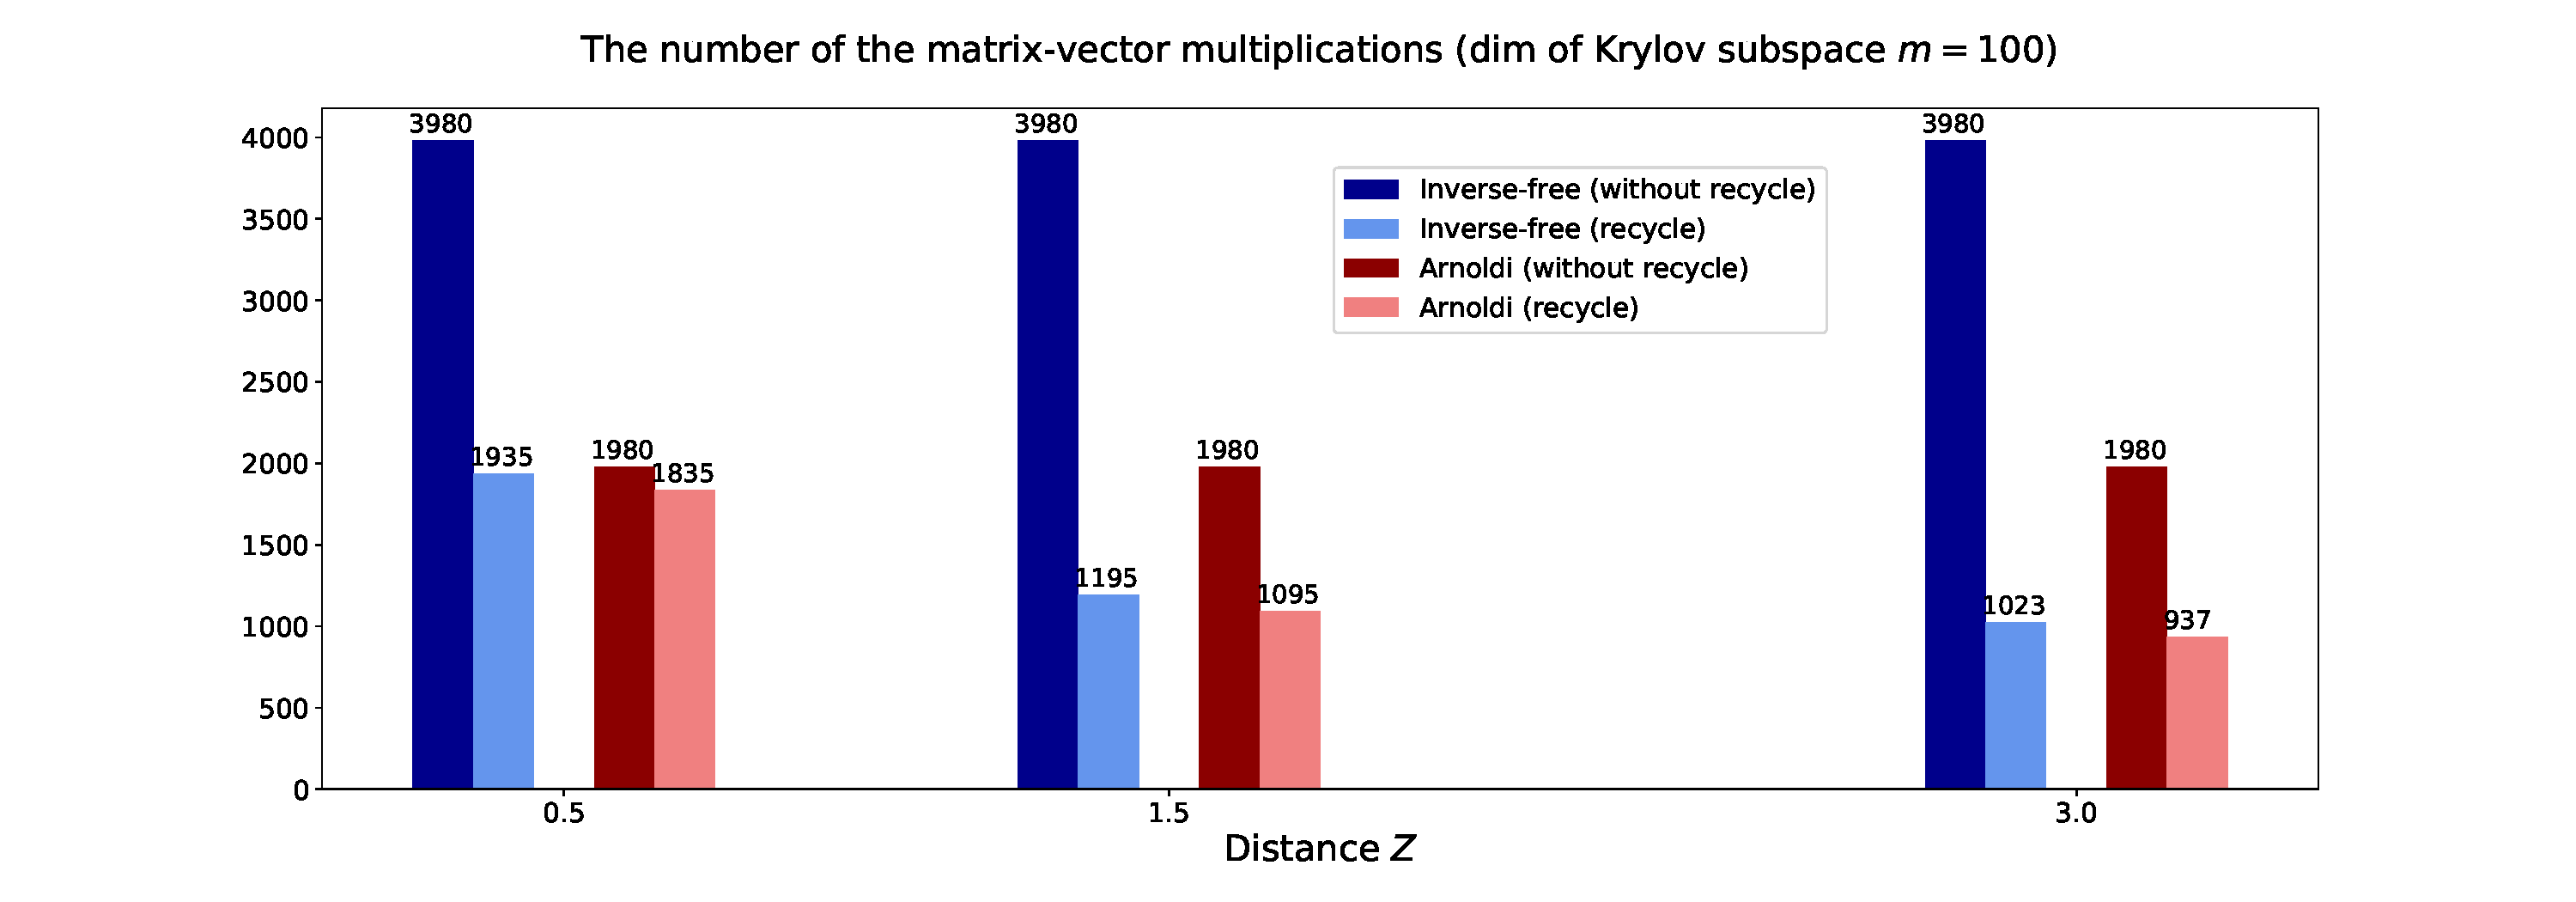
\includegraphics[scale = 0.4]{figures/matvec_100.pdf}
    \caption{The number of the matrix-vector products inside inverse-free and standard Arnoldi methods with or without recycling subspace. The scatterers are two spheres with equal radii $R = 1$ and distance $Z$ is 0.5, 1.5 and 3.0. The dimension of the Krylov subspace is set as $m = 100$.}
    \label{matvec100}
\end{figure}

\begin{figure}[H]
    \centering
    \hspace*{-1.5cm}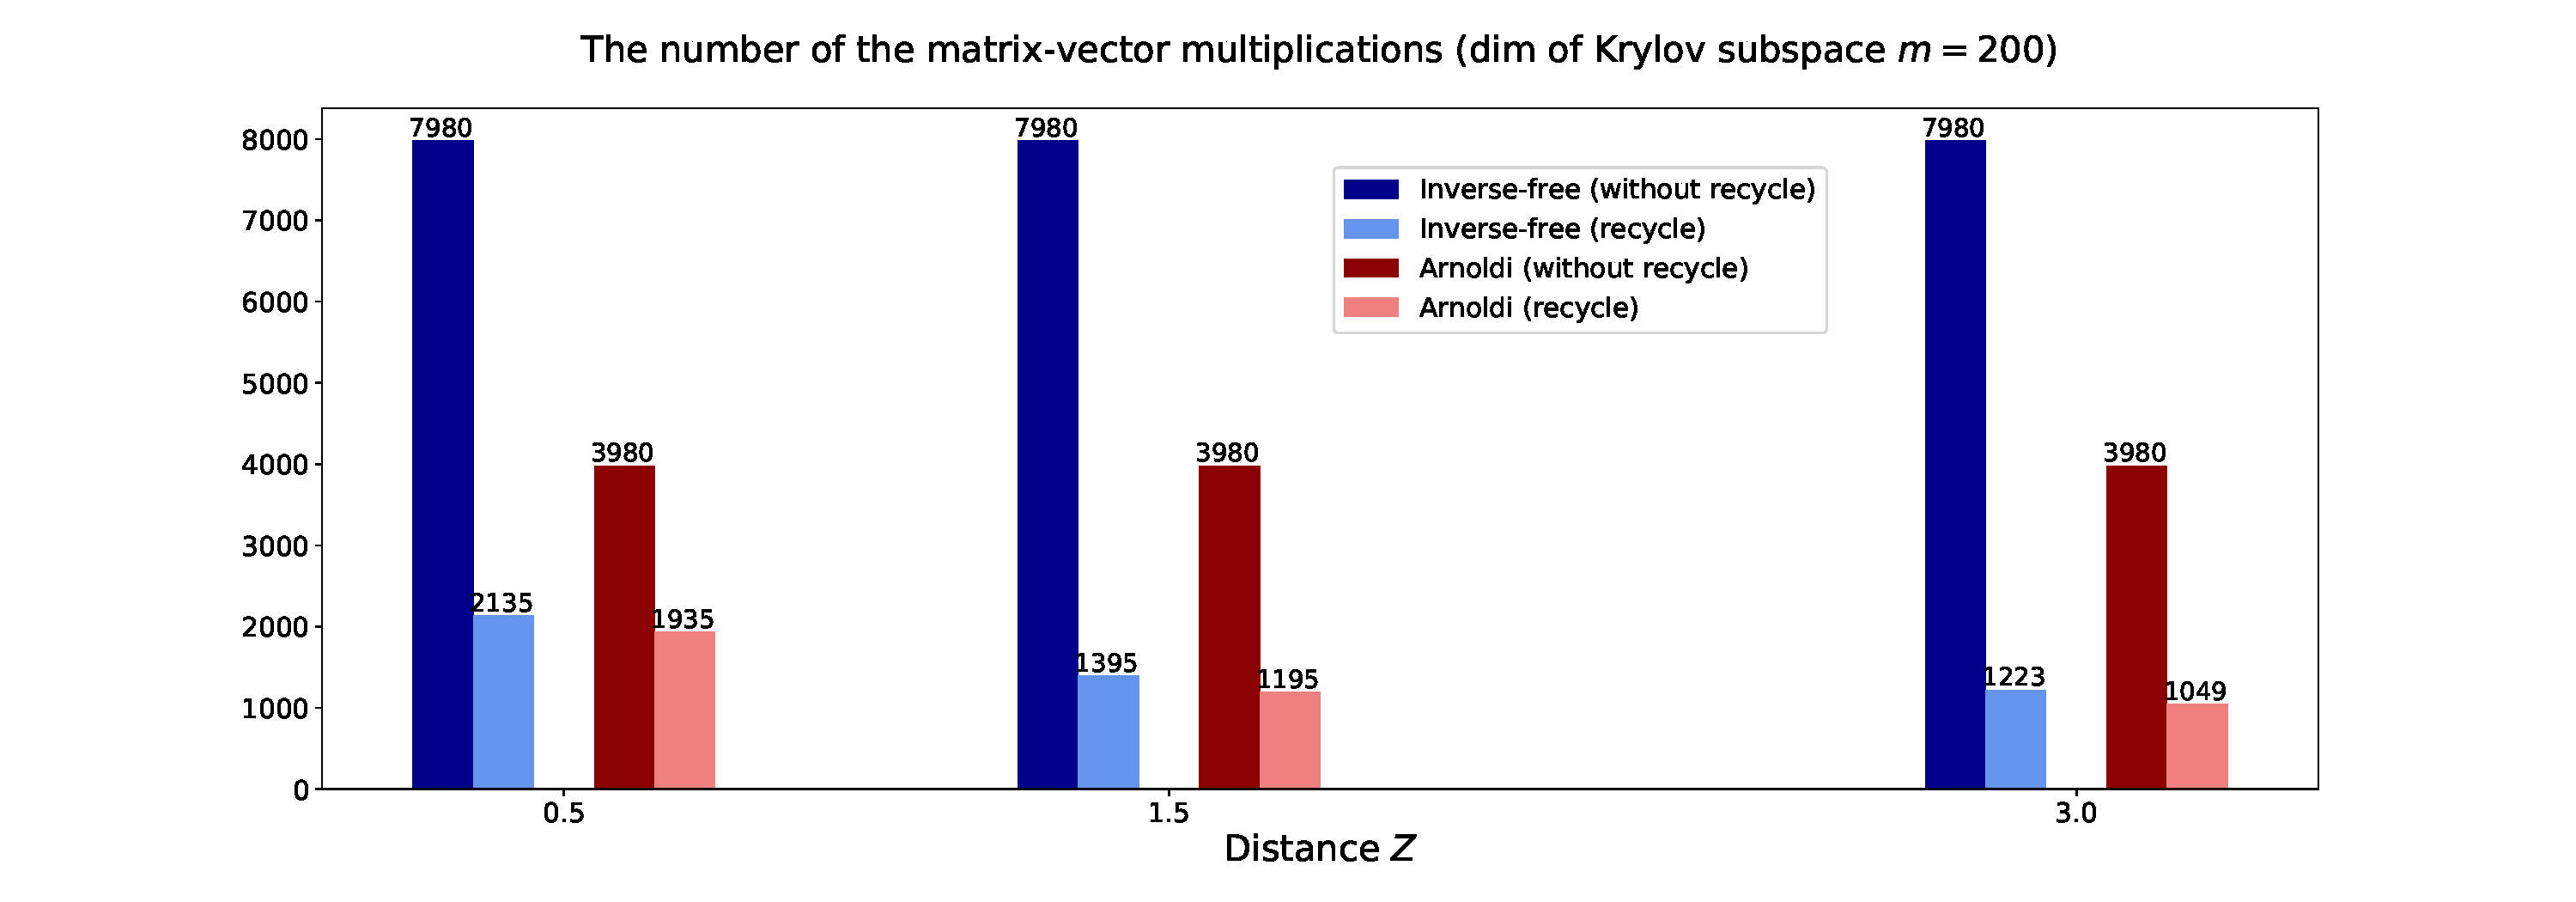
\includegraphics[scale = 0.4]{figures/matvec_200.pdf}
    \caption{The number of the matrix-vector products inside inverse-free and standard Arnoldi methods with or without recycling subspace. The scatterers are two spheres with equal radii $R = 1$ and distance $Z$ is 0.5, 1.5 and 3.0. The dimension of the Krylov subspace is set as $m = 200$.}
    \label{matvec200}
\end{figure}

%Note that for the recycled methods Algorithm \ref{Alg for computing the evals kry recycled}-\ref{Alg for computing the evals arno recycled}
%we apply different rules for extracting the eigenvectors. For  
%is different which depends on the 

%For the standard Arnoldi method,  it can be noticed that the number of FLOP is cubicly increasing with the size of the matrix 
%no matter the subspace is recycled or not. For the inverse-free Krylov subspace methods, as the wavenumber $k$ increases, the number of the extreme eigenvalues
%decreases which makes the number of extracted eigenvectors decreases as well. Therefore, for the large-scale problems, the inverse-free Krylov subspace method with 
%subspaces recycled would be applied to compute the Casimir energy with lower complexity and desired accuracy.
